\section{Experimente}


\iffalse
\begin{frame}{Programmablauf}
    \begin{itemize}
        \item Algorithmen in C++
        \begin{itemize}
            \item effizient
            \item Fluss-Libary (Lemon \footfullcite{Lemon-Lib})
        \end{itemize}
        \item testen und Datenverwaltung in Python
        \begin{itemize}
            \item data analysis Libary (Pandas)
            \item plotting
        \end{itemize}
        \item Subsamples von Python in C++ Skripte
    \end{itemize}

\end{frame}
\fi



\begin{frame}{Implementierung der Testumgebung}
    \begin{minipage}[t]{0.44\textwidth}
        \begin{itemize}
            \item Algorithmen in C++
            \begin{itemize}
                \item effizient
                \item Graph-Library (Lemon \footfullcite{Lemon-Lib})
            \end{itemize}
            \item Testen und Datenverwaltung in Python
            \begin{itemize}
                \item data analysis Library (Pandas)
                \item plotting
            \end{itemize}
            \item Subsamples von Python in C++ Skripte
        \end{itemize}
    \end{minipage}
    \hfill
    \begin{minipage}[t]{0.55\textwidth}
        \begin{center}
            \vspace{-\baselineskip} % Move image to the top
            % Flussdiagram Der Pipeline
            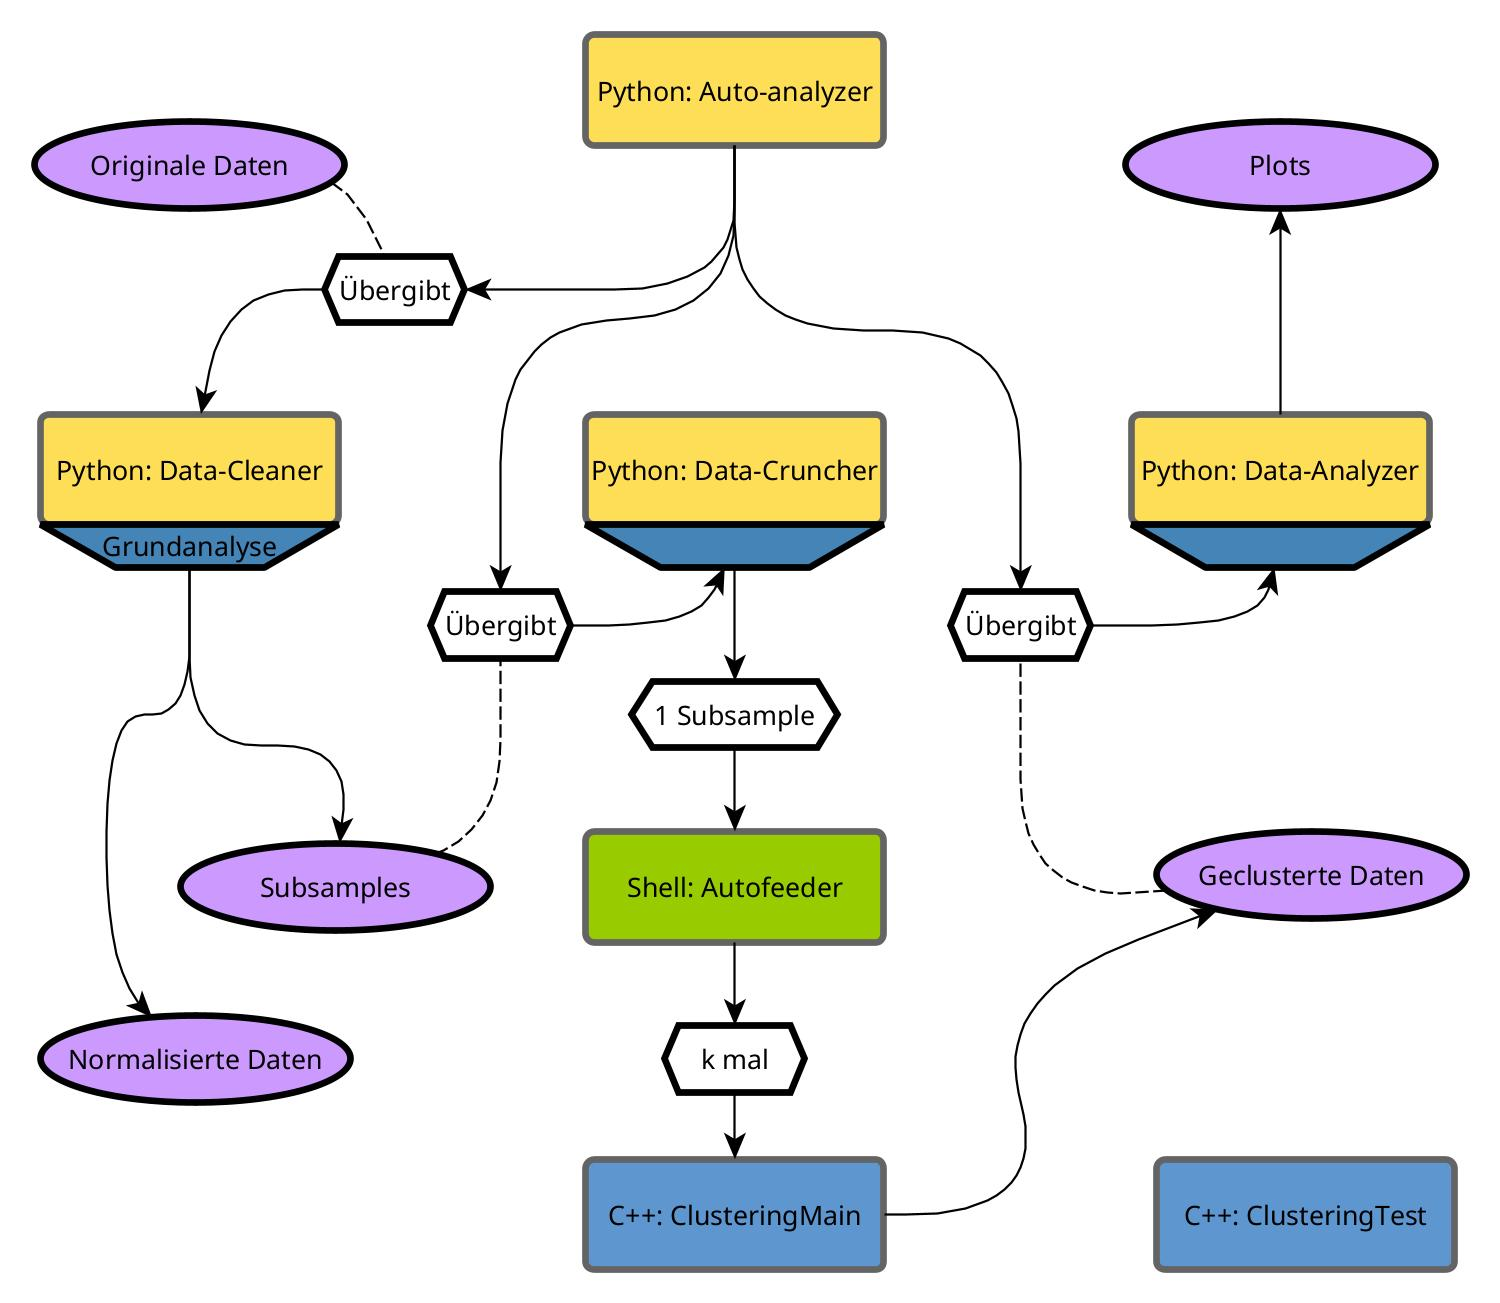
\includegraphics[width=\textwidth*6/7]{fig/Analyse-Flowchart/Flow-Chart.jpg}
        \end{center}   
    \end{minipage}
\end{frame}





















\begin{frame}{Laufzeitenvergleich}
    \begin{minipage}[t]{0.49\textwidth}
        \begin{large}
            \begin{center}
                Laufzeit Red-Clustering
            \end{center}
        \end{large}        
        %\vspace{-\baselineskip} % Move image to the top
        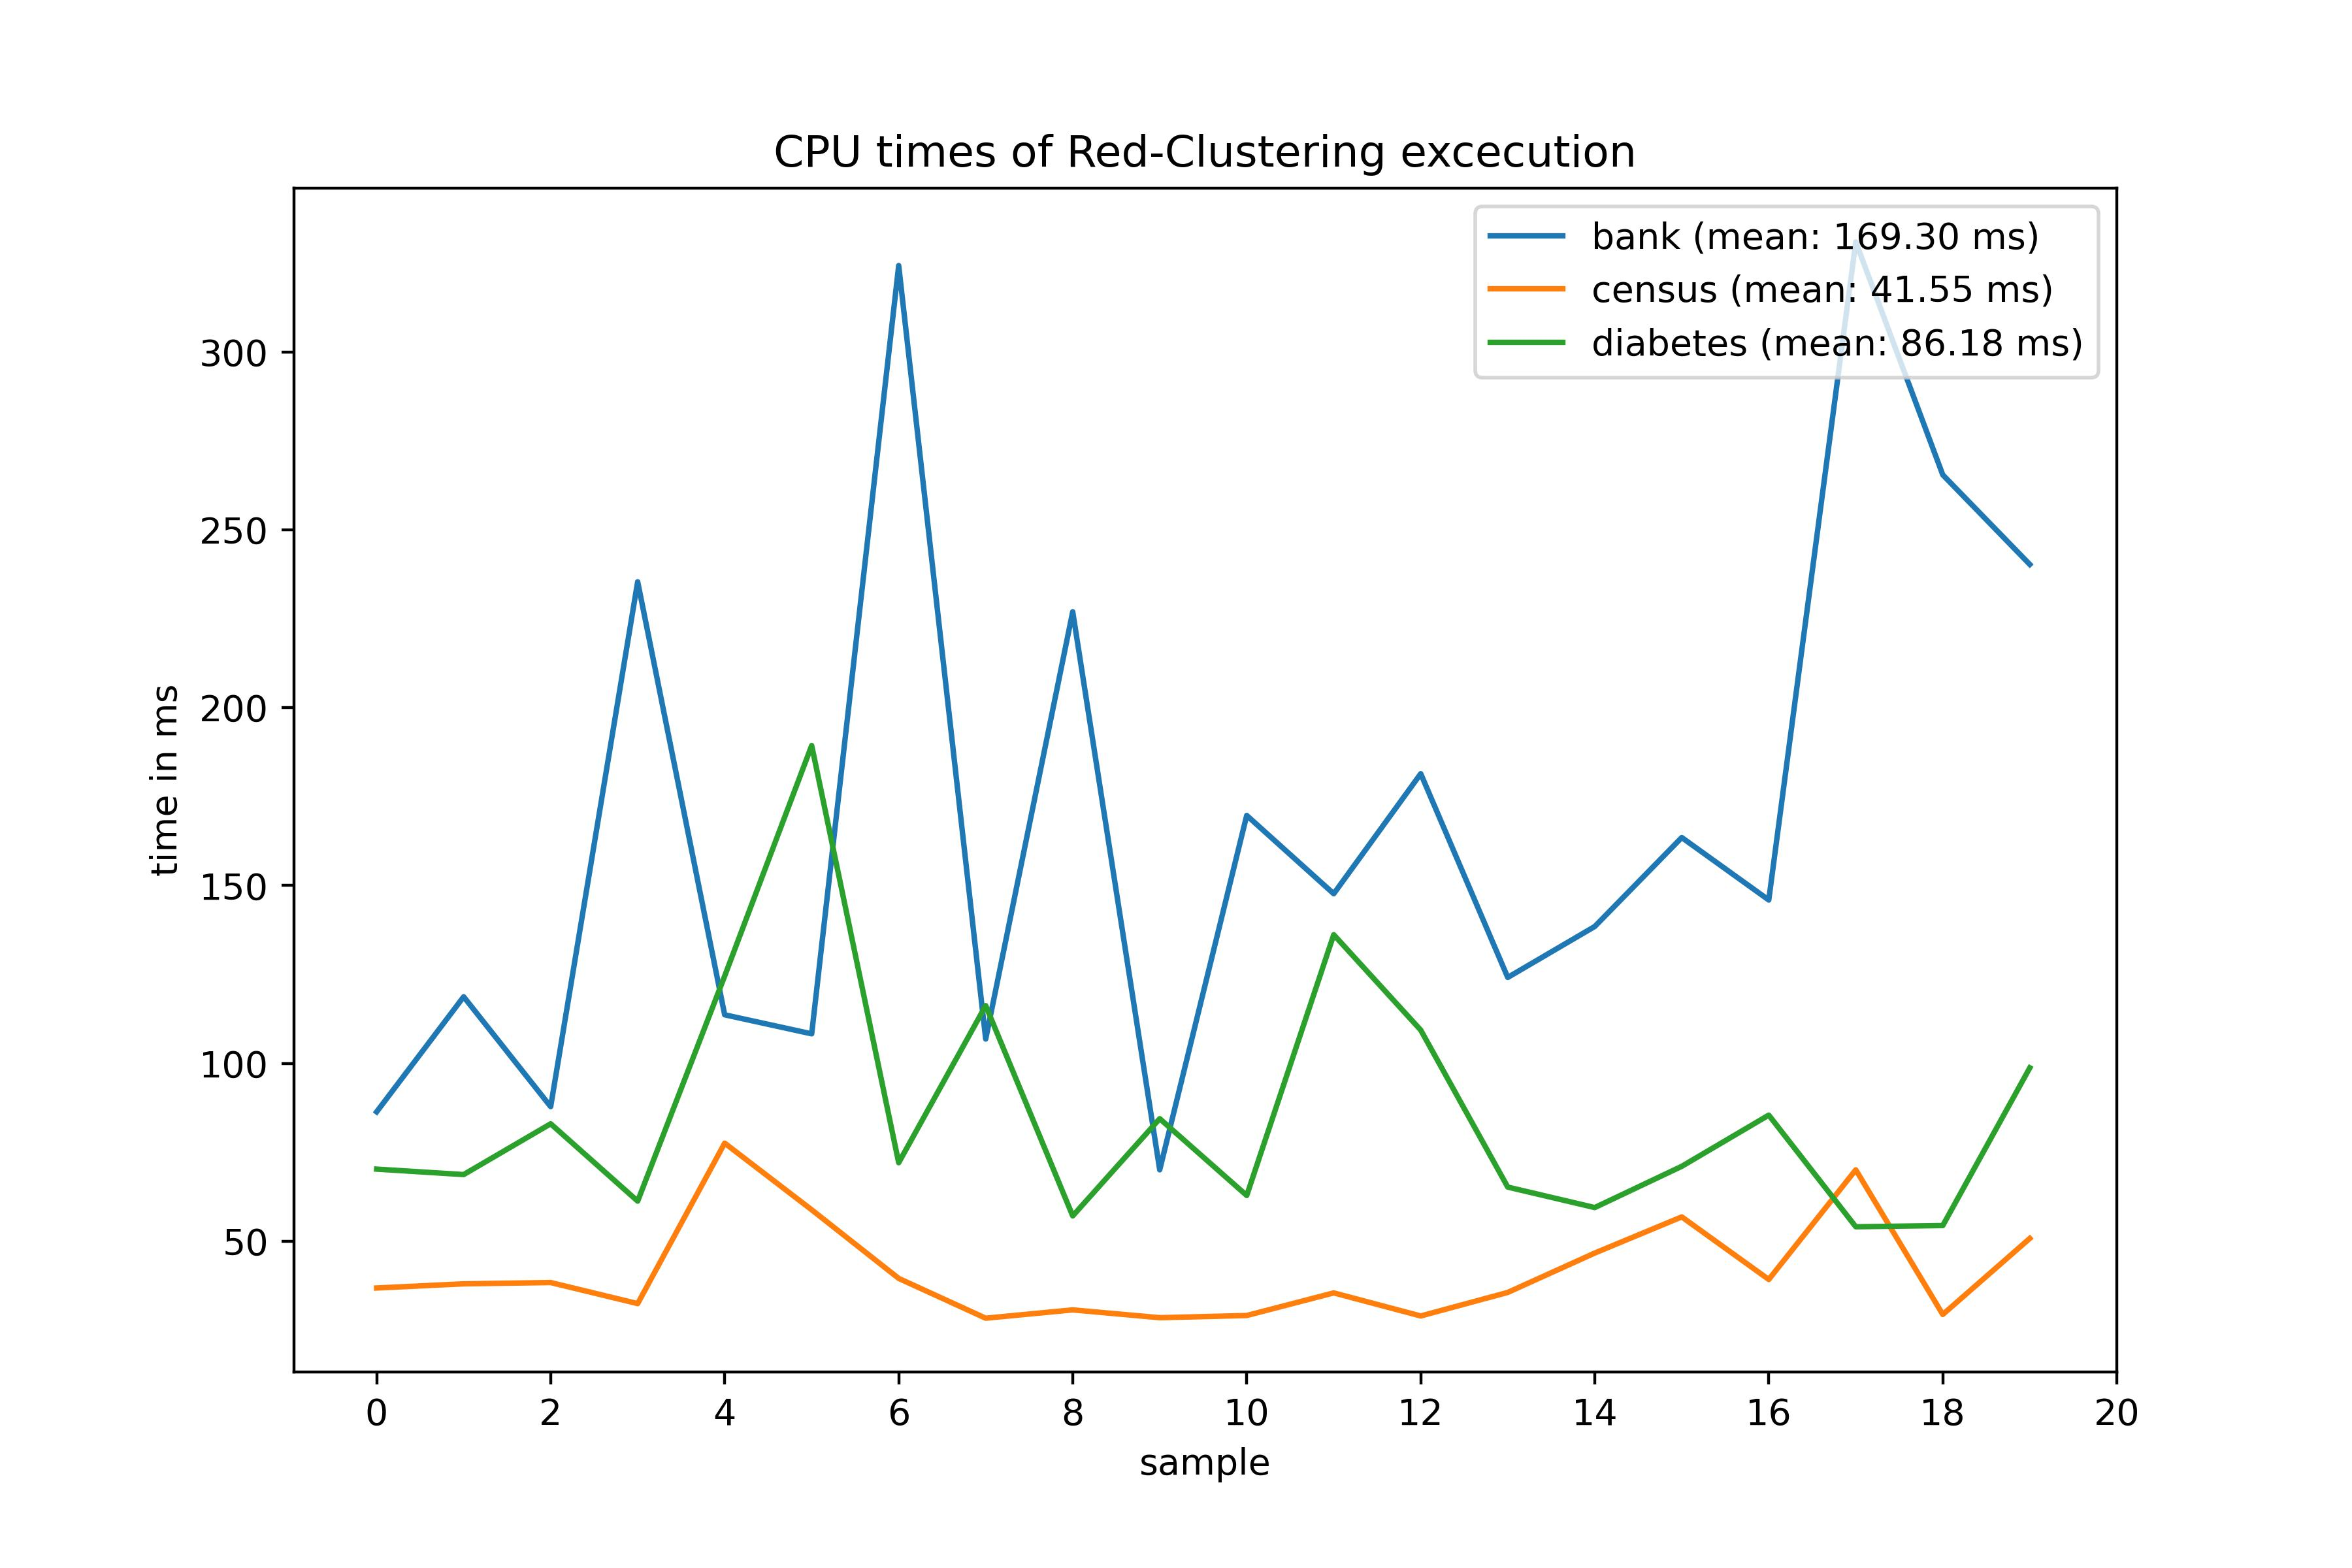
\includegraphics[width=\textwidth]{fig/Runtime/Timinganalysis Red-Clustering.jpg}
    \end{minipage}
    \hfill
    \begin{minipage}[t]{0.49\textwidth}
        \begin{large}
            \begin{center}
                Laufzeit Fast-Anchor-Clustering
            \end{center}
        \end{large}
        %\vspace{-\baselineskip} % Move image to the top
        
\includegraphics[width=\textwidth]{fig/Runtime/Timinganalysis Fast-Clustering.jpg}
    \end{minipage}
\end{frame}










\iffalse
\begin{frame}{Güteauswertung - Bankdaten}
    \begin{center}
        %\begin{large}
        %    Clustergrößen der Bankdaten
        %\end{large}
        \vspace{-\baselineskip} % Move image to the top
        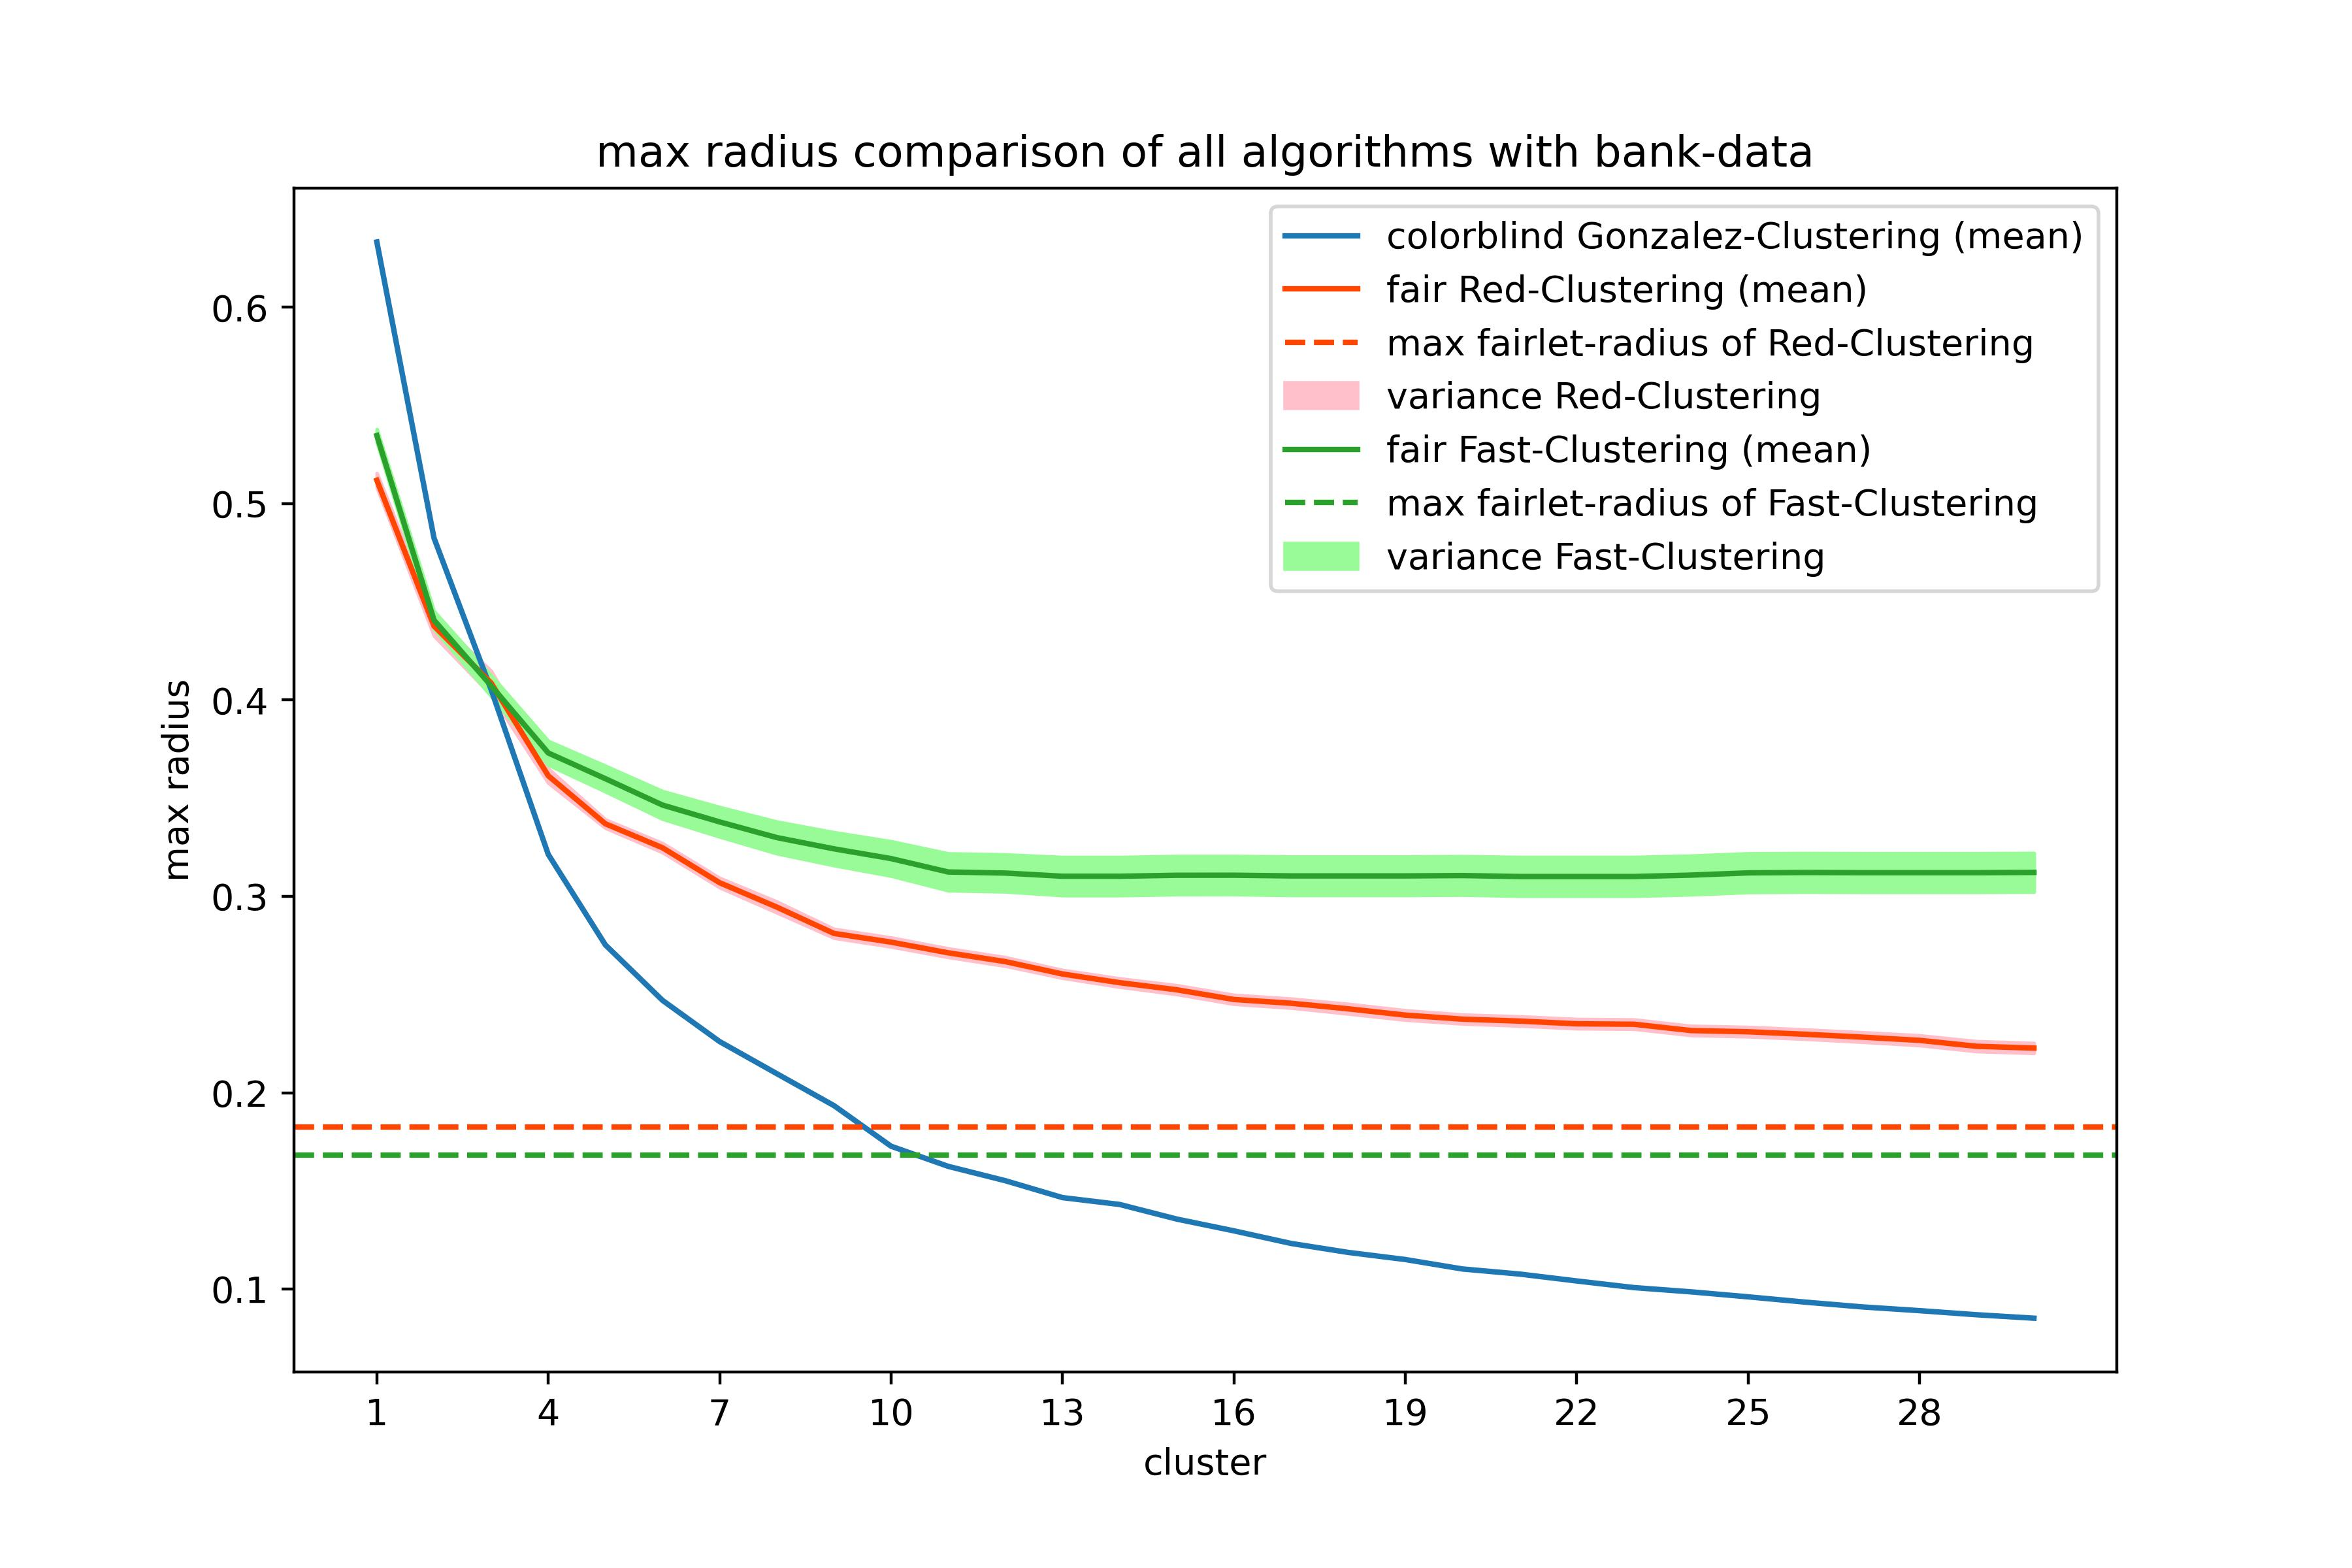
\includegraphics[height=\textheight*4/5]{fig/Clustersizes/Collective Analysis bank(Cluster-30).jpg}
    \end{center}
\end{frame}
\fi 

\begin{frame}{Güteauswertung}
    \begin{minipage}[t]{0.49\textwidth}
        \begin{large}
            \begin{center}
                Bankdaten
            \end{center}
        \end{large}        
        %\vspace{-\baselineskip} % Move image to the top
        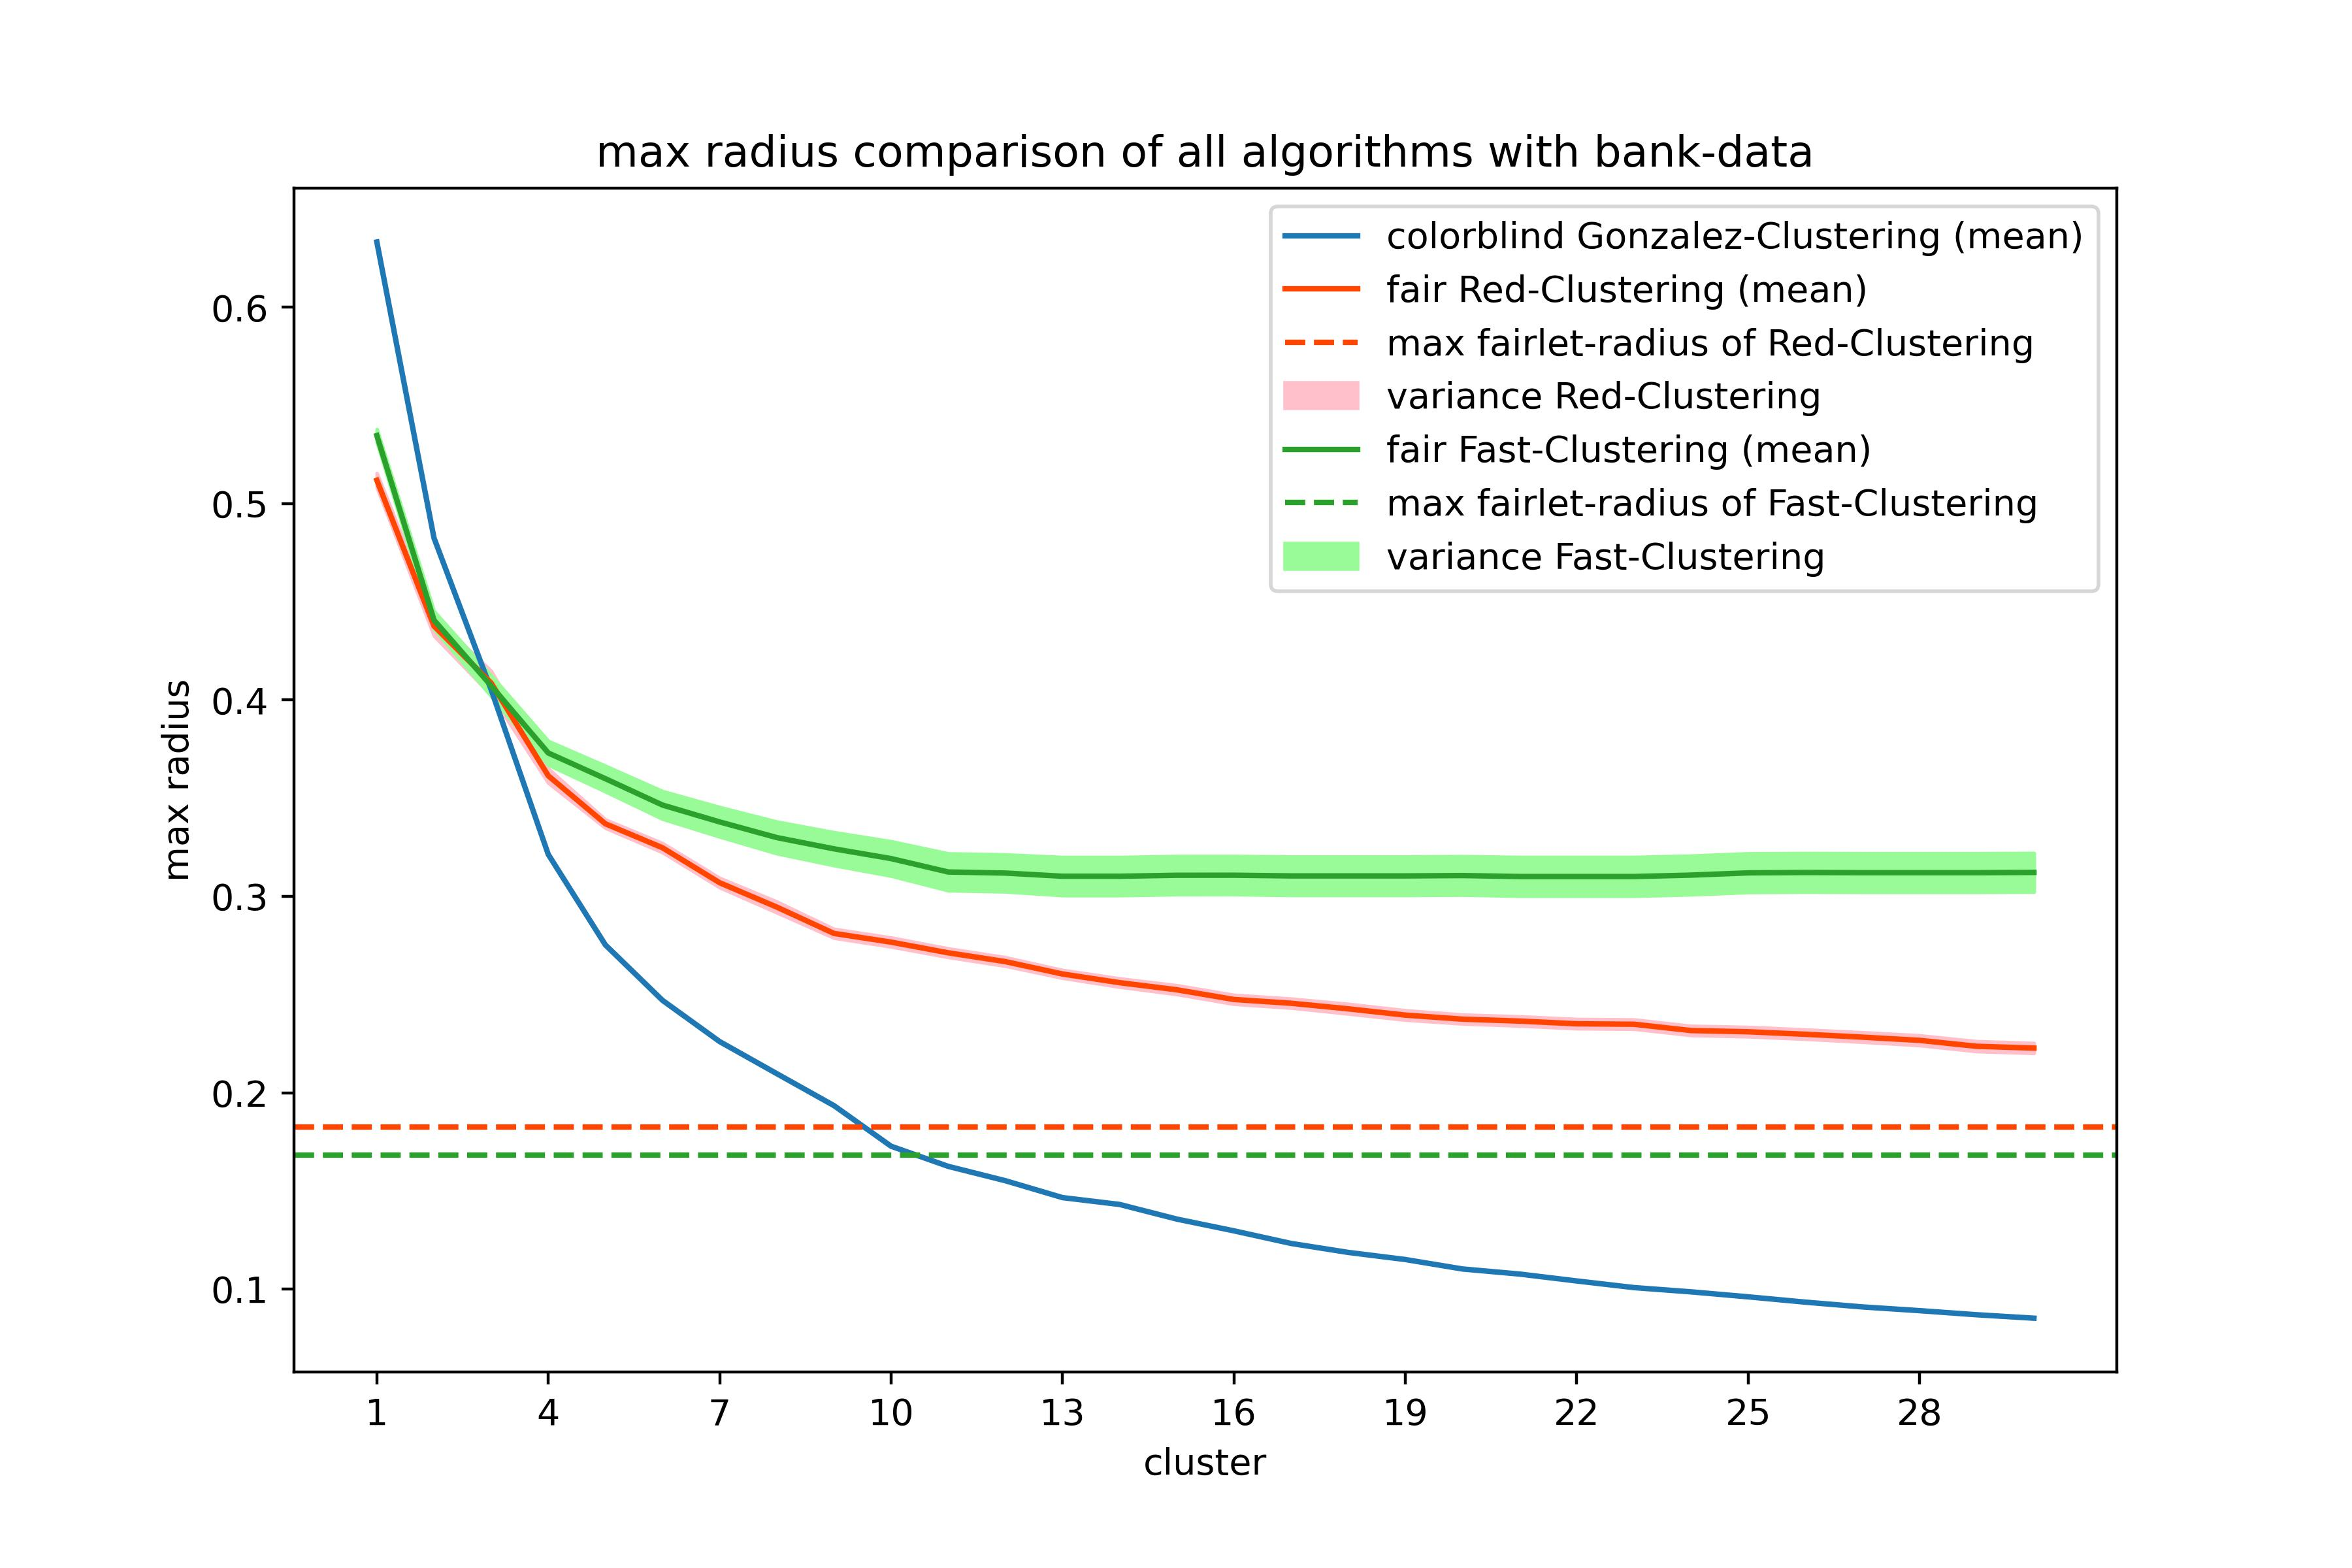
\includegraphics[width=\textwidth]{fig/Clustersizes/Collective Analysis bank(Cluster-30).jpg}
    \end{minipage}
    \hfill
    \begin{minipage}[t]{0.49\textwidth}
        \begin{large}
            \begin{center}
                Zensusdaten
            \end{center}
        \end{large}
        %\vspace{-\baselineskip} % Move image to the top
        
\includegraphics[width=\textwidth]{fig/Clustersizes/Collective Analysis census(Cluster-30).jpg}
    \end{minipage}
\end{frame}



\begin{frame}{Güteauswertung}
    \begin{center}
        \begin{minipage}[t]{0.55\textwidth}
            \begin{center}
                \begin{large}
                    Diabetesdaten
                \end{large} 
            \end{center}   
            %\vspace{-\baselineskip} % Move image to the top
            
\includegraphics[width=\textwidth]{fig/Clustersizes/Collective Analysis diabetes(Cluster-30).jpg}
        \end{minipage}
    \end{center}
\end{frame}





